\documentclass[a4paper]{article}
\usepackage[final]{pdfpages}

\addtolength{\textheight}{3cm}
\addtolength{\voffset}{-.8cm}

\begin{document}
\pagenumbering{arabic}
\setcounter{page}{1}

\title{Curso 2: Generaci\'on de Lenguaje Natural y Aplicaciones}
\author{Carlos Areces\\
  {\tt carlos.areces@gmail.com} 
\and 
Luciana Benotti\\
  {\tt Luciana.Benotti@gmail.com} \\
 \ \\
  Equipo TALARIS - INRIA Nancy Grand Est - Francia\\
  Equipo PLN - Universidad Nacional de C\'ordoba - Argentina
}


\maketitle

Este curso est\'a compuesto por dos partes. En la primera se dar\'a una introducci\'on al problema de generaci\'on de lenguaje natural. Presentaremos los algoritmos cl\'asicos de generaci\'on, haciendo \'enfasis en la generaci\'on de referencias. En la segunda parte discutiremos sistemas de generaci\'on situados en un entorno virtual.

La segunda parte tiene como requisito previo la primera. La evaluaci\'on final cubrir\'a temas de ambas partes.

\section{Introducci\'on a la Generaci\'on de Lenguaje Natural}

\paragraph{Profesor:} Carlos Areces (INRIA Grand Est, Francia / Univ. Nacional de C\'ordoba)

\paragraph{Horario:} Lunes, martes y mi\'ercoles de 14 a 17 hs (9 horas de clase)

\paragraph{Pre-requisitos:} Conocimientos b\'asicos de l\'ogica y algoritmos. No se asume conocimiento previo de procesamiento de lenguaje natural.

\paragraph{Resumen:} El problema de generaci\'on de lenguaje natural puede definirse, intuitivamente, como el proceso de transformaci\'on de informaci\'on en texto (escrito o hablado) en lenguaje natural (por ejemplo, Ingl\'es o Español). El texto generado debe ser no solamente gramaticalmente correcto, sino adecuado para el contexto en donde ser\'a utilizado.

\subsection*{Lunes:} El Problema de Generaci\'on de Lenguaje Natural (GLN). Historia. Generaci\'on vs. Parsing. GNL Pipeline. Representaci\'on de Informaci\'on e Inferencia para GLN. Evaluaci\'on de Sistemas de GLN.

\subsection*{Martes:} Generaci\'on Sint\'actica. Generaci\'on via Charts. Tree Adjoining Grammars. Interface Sint\'actica-Sem\'antica.

\subsection*{Mi\'ercoles:} Algoritmos de Generaci\'on de Expresiones Referenciales. Informaci\'on Proposicional vs. Informaci\'on Relacional. Optimizaci\'on de Algoritmos. Evaluaci\'on.


\section{Generaci\'on de Instrucciones en un Entorno Virtual}

\paragraph{Profesora:} Luciana Benotti (INRIA Grand Est, Francia / Univ. Nacional de C\'ordoba)

\paragraph{Horario:} Jueves y viernes de 14 a 17 hs (6 horas de clase)

\paragraph{Pre-requisitos:} Primera parte

\paragraph{Resumen:} En esta parte del curso nos enfocaremos en sistemas de generaci\'on que tienen como objetivo una tarea concreta y que est\'an situados en un entorno 3D. Analizaremos como estas dos caracter\'isticas tienen impacto en las estrategias de generaci\'on de lenguaje natural.

\subsection*{Jueves:} 

\begin{itemize}
\item Introducci\'on a entornos Virtuales (e.g., Second Life) y Aplicaciones (e.g., Tutoring) como entornos para Sistemas de GNL. 
\item Inferencia Orientada a Metas: Algoritmos de Planning y su uso en Entornos Virtuales (Russell and Norvig, 2003). 
\end{itemize}

\subsection*{Viernes:} 
\begin{itemize}
\item Generaci\'on de Referencias en un Entorno Virtual: Estrategias de Referencia (Stoia et al, 2006).
\item Supervisi\'on de la Interpretaci\'on: Evaluaci\'on (Byron et al, 2009).  
\end{itemize}

\subsection*{Bibliograf\'ia:}
\begin{enumerate}
\item Stuart Russell and Peter Norvig (2003). Artificial Intelligence: A Modern Approach (Segunda Edici\'on). Prentice Hall. Secciones: 11.1, 11.2, 11.4, 11.7. Ver pag.~\pageref{planning-state-search}. \\
\textbf{Contenido:} Este cap\'itulo es una buena introducci\'on al \'area de planning tomado de uno de los libros cl\'asicos en el mundo para la ense\~nanza de inteligencia artificial. La Secci\'on 11.1 introduce planning como un problema de inferencia e ilustra su uso con ejemplos. La Secci\'on 11.2 presenta los algoritmos de planning de b\'usqueda en el espacio de estados (forward-chaining, backward chaining y uso de heur\'isitcas). La Secci\'on 11.4 introduce el algoritmo graphplan. La Secci\'on 11.7 presenta un resumen de los conceptos principales as\'i como una discusi\'on de la evoluci\'on hist\'orica del \'area de planning.  
\item Laura Stoia, Darla Magdalene Shockley, Donna Byron, and Eric Fosler-Lussier. Noun phrase generation for situated dialogs. In Proc. of the 4th International Natural Language Generation Conference (INLG 2006), pages 81-88, Sydney, Australia, 2006. Association for Computational Linguistics. Ver pag.~\pageref{give-challenge}.\\
\textbf{Contenido:} Este art\'iculo presenta el problema de generaci\'on de expresiones referenciales situado en un entorno virtual. La generaci\'on de expresiones referenciales cl\'asica (es decir, no situada) asume que el entorno de referencia es est\'atico. Este art\'iculo explora el caso en el que no se asume esta simplificaci\'on, es decir el caso en el que el entorno puede cambiar y estos cambios pueden ser aprovechados para hacer el proceso de referencia mas efectivo. 
\item Donna Byron, Alexander Koller, Kristina Striegnitz, Justine Cassell, Robert Dale, Johanna Moore, and Jon Oberlander. Report on the First NLG Challenge on Generating Instructions in Virtual Environments (GIVE). In Proc. of the 12th European Workshop on Natural Language Generation (ENLG 2009), Athens, Greece. Association for Computational Linguistics. Ver pag.~\pageref{situated-REG}. \\
\textbf{Contenido:} Este art\'iculo presenta el \textit{GIVE Challenge}. El \textit{GIVE Challenge} es un desaf\'io propuesto por el grupo de inter\'es especial en GLN (SIGGEN) de la Asociaci\'on de Lingu\'istica Computacional (ACL) para evaluar sistemas de GLN situados en un entorno virtual. El art\'iculo discute distintas m\'etricas de evaluaci\'on para este tipo de sistemas. 
\end{enumerate}

\pagebreak
\label{planning-state-search} 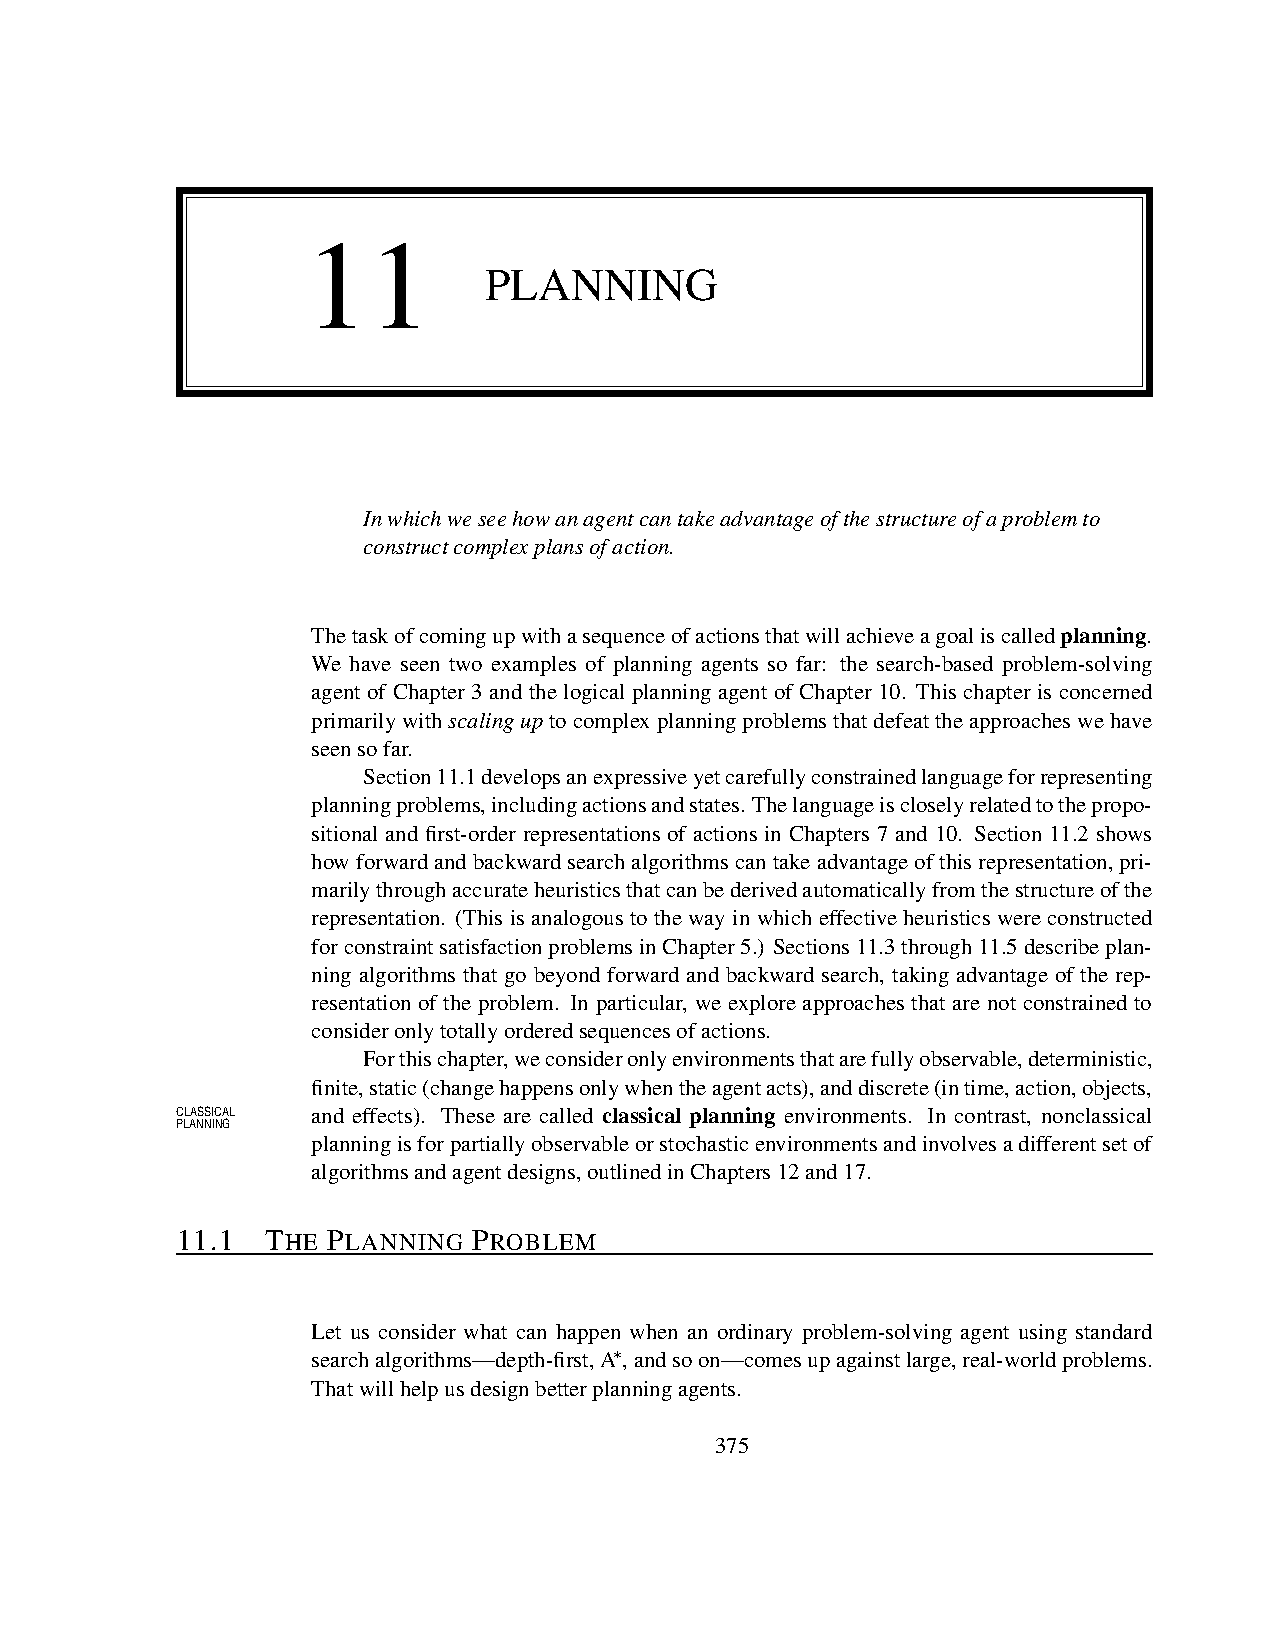
\includepdf[nup=1x2, landscape, pages={1-13}, scale=.92, frame, pagecommand={}]{russell-norvig-chap11.pdf}
\label{planning-graphplan} \includepdf[nup=1x2, landscape, pages={21-28}, scale=.92, frame, pagecommand={}]{russell-norvig-chap11.pdf}
\label{planning-history} \includepdf[nup=1x2, landscape, pages={34-38}, scale=.92, frame, pagecommand={}]{russell-norvig-chap11.pdf}
\label{give-challenge} 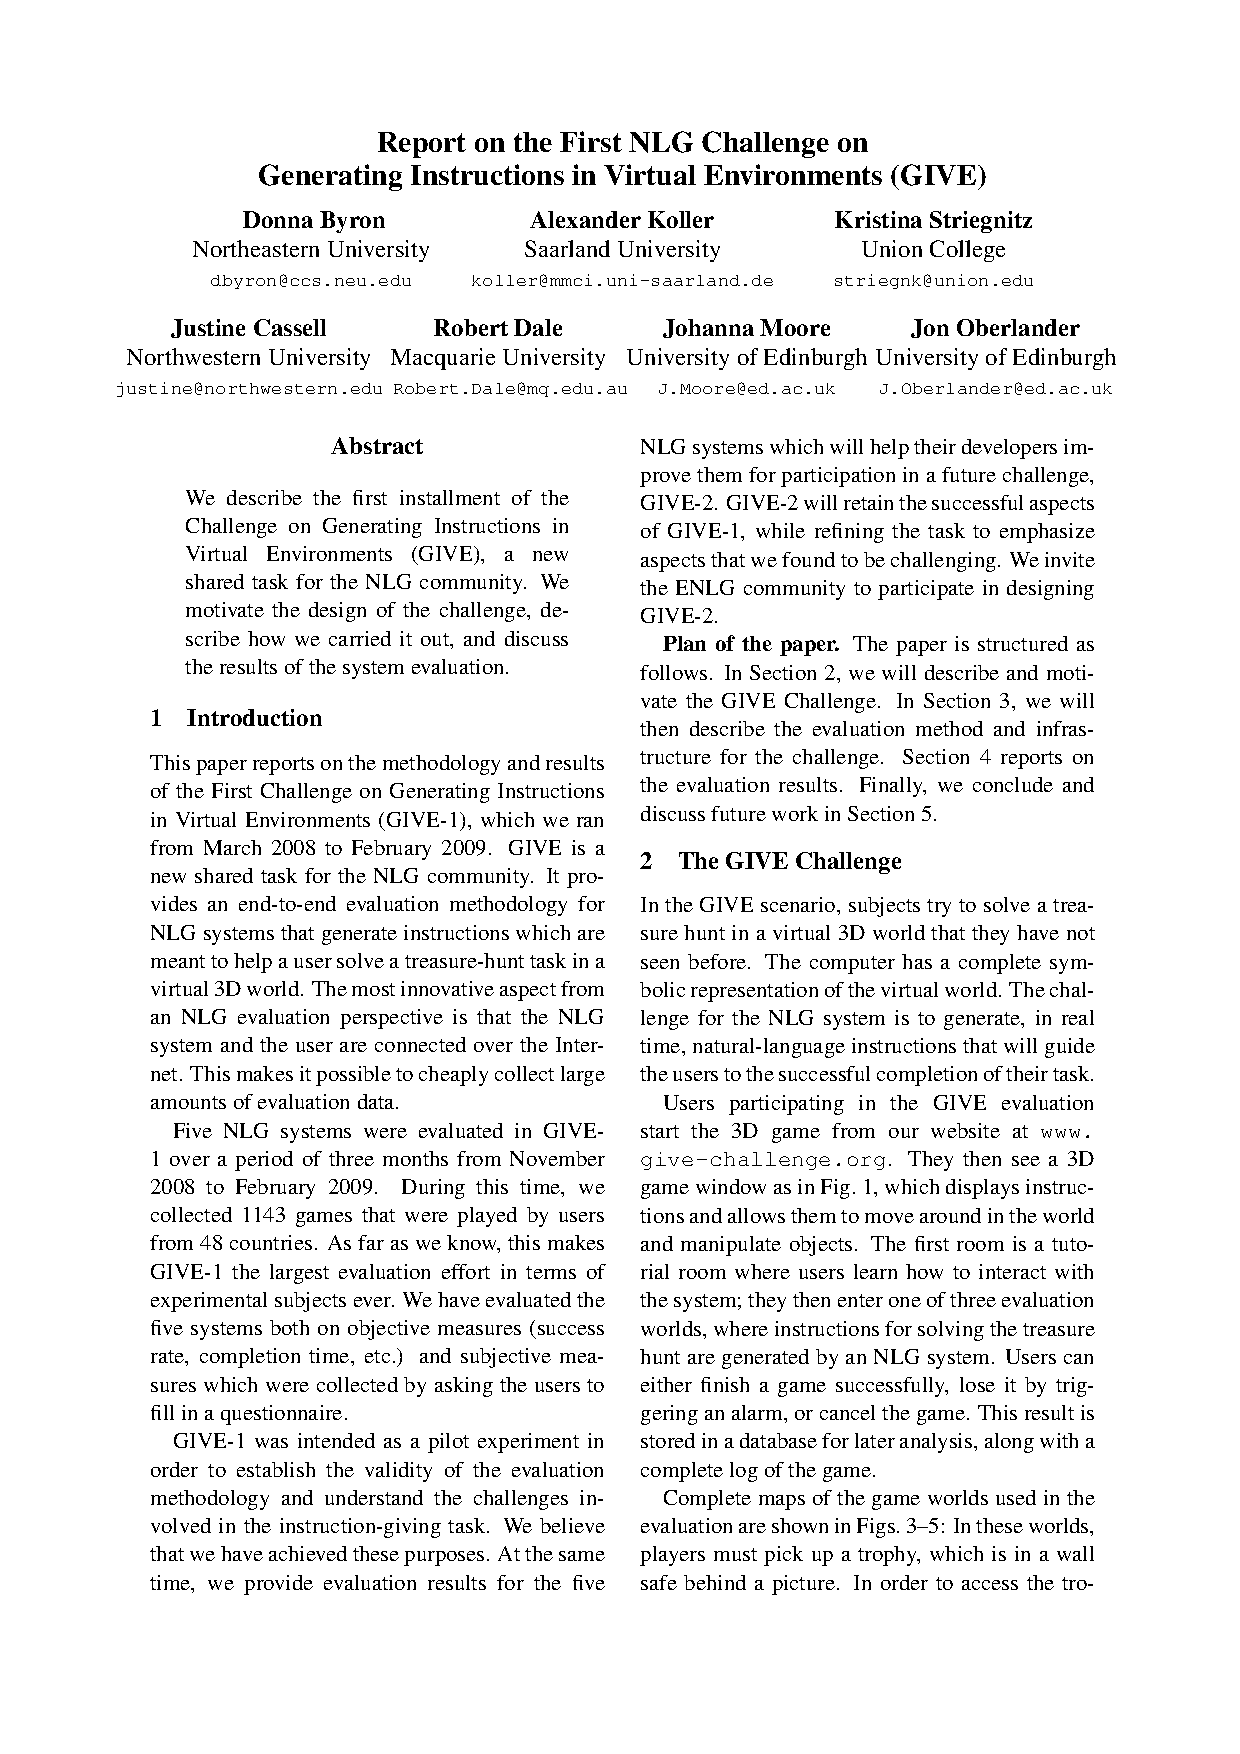
\includepdf[pages={1-9}, scale=.92, frame, pagecommand={}]{give-report-09.pdf}
\label{situated-REG} 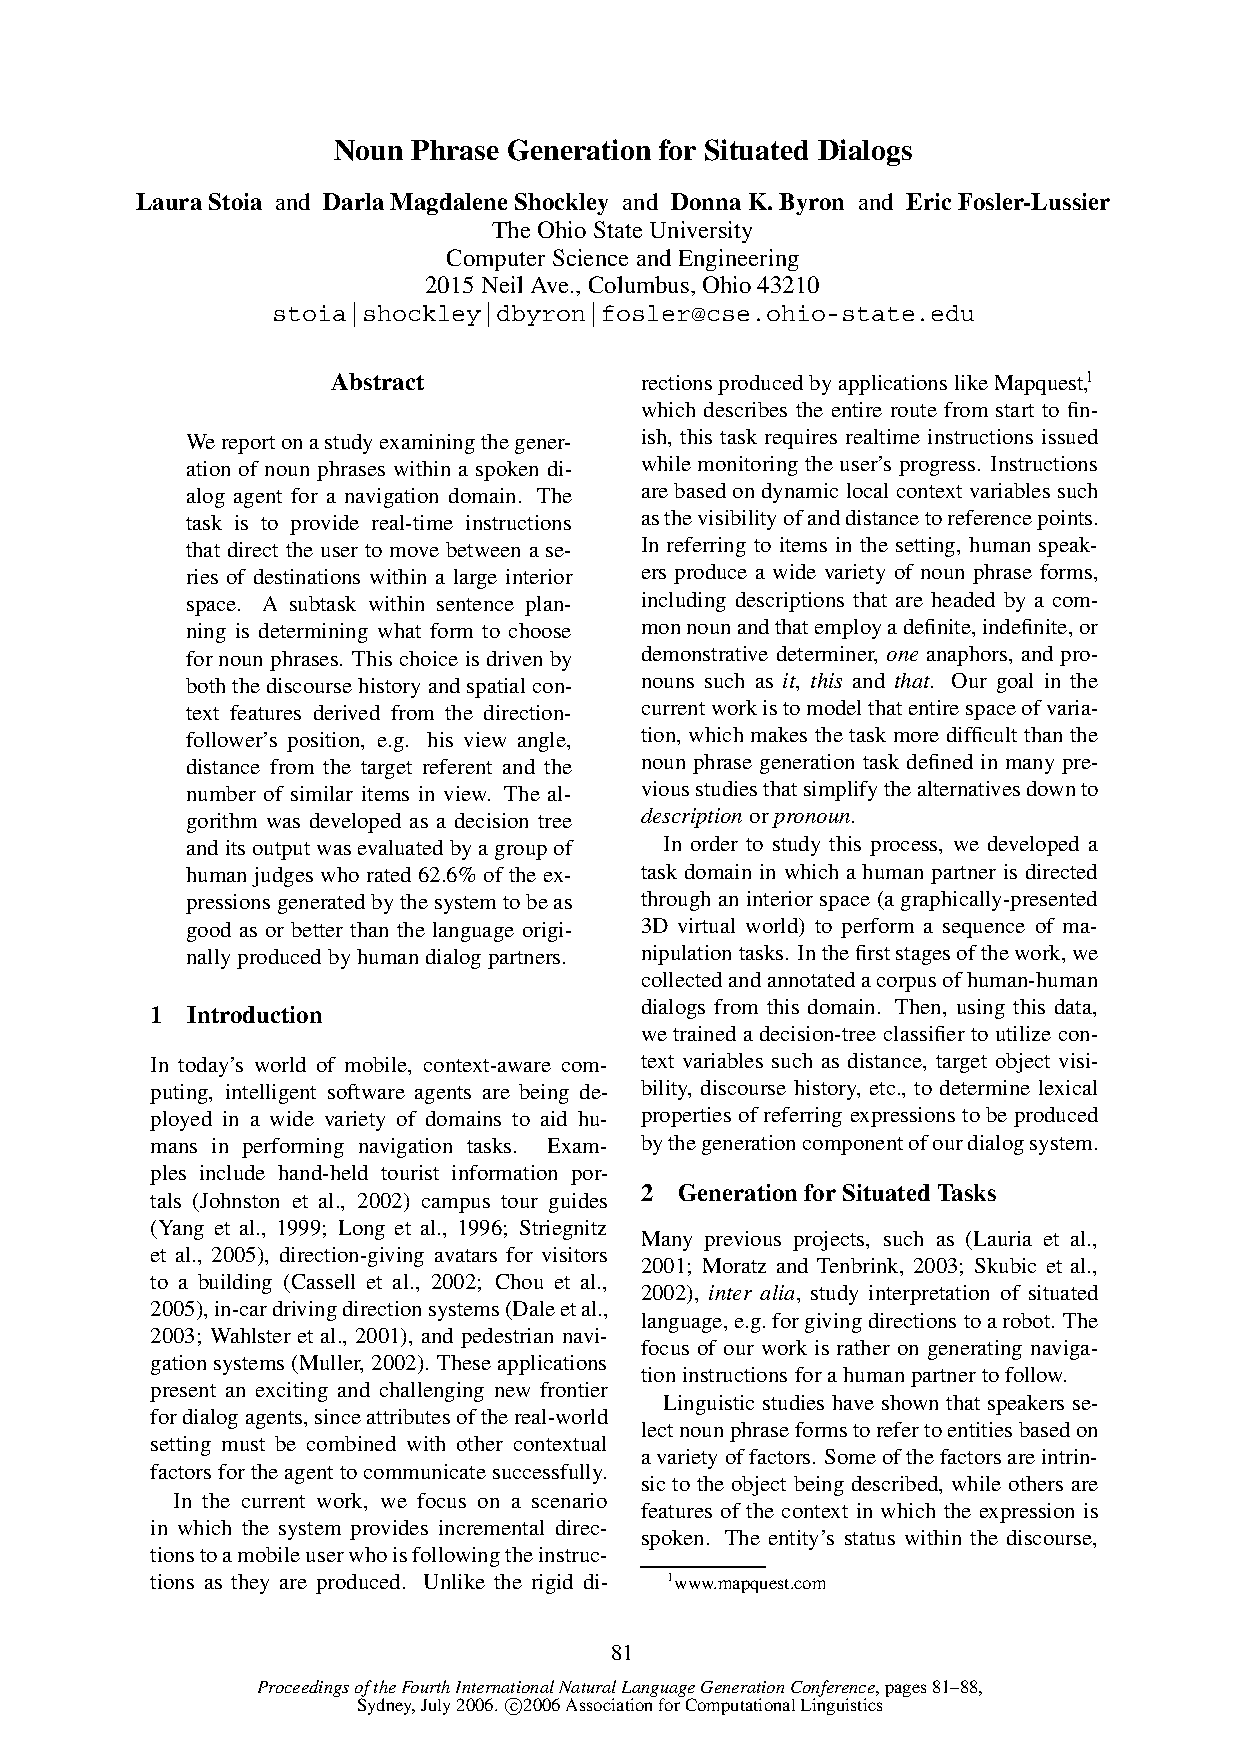
\includepdf[pages={1-8}, scale=.92, frame, pagecommand={}]{Situated-REG.pdf}

\end{document}
